%% LyX 2.2.2 created this file.  For more info, see http://www.lyx.org/.
%% Do not edit unless you really know what you are doing.
\documentclass[english]{article}
\usepackage[T1]{fontenc}
\usepackage[latin9]{luainputenc}
\setlength{\parskip}{\smallskipamount}
\setlength{\parindent}{0pt}
\usepackage{babel}
\usepackage{graphicx}
\usepackage[unicode=true,
 bookmarks=true,bookmarksnumbered=false,bookmarksopen=false,
 breaklinks=false,pdfborder={0 0 1},backref=false,colorlinks=false]
 {hyperref}
\hypersetup{pdftitle={Power Enjoy: Design Document},
 pdfauthor={Niccolo' Raspa, Matteo Marinelli}}

\makeatletter

%%%%%%%%%%%%%%%%%%%%%%%%%%%%%% LyX specific LaTeX commands.
%% Because html converters don't know tabularnewline
\providecommand{\tabularnewline}{\\}

%%%%%%%%%%%%%%%%%%%%%%%%%%%%%% Textclass specific LaTeX commands.
\newenvironment{lyxlist}[1]
{\begin{list}{}
{\settowidth{\labelwidth}{#1}
 \setlength{\leftmargin}{\labelwidth}
 \addtolength{\leftmargin}{\labelsep}
 \renewcommand{\makelabel}[1]{##1\hfil}}}
{\end{list}}
\newcommand{\strong}[1]{\textbf{#1}}

%%%%%%%%%%%%%%%%%%%%%%%%%%%%%% User specified LaTeX commands.
\usepackage{changepage}

\makeatother

\begin{document}

\title{\emph{Power EnJoy \\
Integration Test Plan Document}\\
\vspace{12px}}

\author{Niccolo' Raspa, Matteo Marinelli}

\maketitle
\vspace*{20px}
\begin{center}
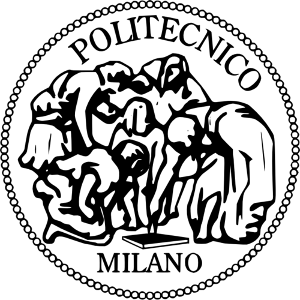
\includegraphics[scale=0.6]{../DD/images/polimi} 
\par\end{center}

\vspace{100px}
\begin{center}
Software Engineering 2 Course Project
\par\end{center}

\pagebreak{}

\section*{ASSIGNMENT INFO}

The Integration Test Plan Document (ITPD) aims at describing how you
plan to accomplish the integration test. This document is supposed
to be written before the integration test really happens. Often it
is written in parallel to the Design Document and takes the architectural
description of the software system as a starting point. This document
needs to explain to the development team what to test, in which sequence,
which tools are needed for testing (if any), and which stubs/drivers/oracles
need to be developed. The structure we suggest for this document is
the following (if you introduce changes to this structure, please
provide a justification for this):\pagebreak{}

\tableofcontents{}

\pagebreak{}

\section{Introduction}

\subsection{Revision History}

\begin{table}[!tph]
\begin{tabular}{|c|c|c|c|}
\hline 
Version & Date & Author(s) & Summary\tabularnewline
\hline 
\hline 
1.0 & 06/01/2016 & Niccolo' Raspa, Matteo Marinelli & Initial Release\tabularnewline
\hline 
\end{tabular}

\end{table}


\subsection{Purpose and Scope}

This document represents the Integration Testing Plan Document for
PowerEnJoy. The main purpose of this document is to outline, in a
clear and comprehensive way, the main aspects concerning the organization
of the integration testing activity for all the components that make
up the system. 

This process is essential because it not only guarantees that every
component behaves as expected but also that all the components interoperate
correctly together to fullfil all the functionalities expected from
the system. 

We will focus deeply on the Application Layer since it implements
all the core of our business. This component is divided in different
services which provides great benefits but the implicit granularity
of a service oriented approach must be fully tested to guarantee that
all the subcomponents behave as one cohesive layer.

\paragraph{This document is structured as follows:}
\begin{description}
\item [{Chapter\ 1}] Provides general information about the ITPD document.
\item [{Chapter\ 2}] Explains in details the chosen integration strategy.
In more details:
\end{description}
\begin{itemize}
\item Lists of the subsystems and their subcomponents involved in this process
\item Specifies the criteria that must be met before integration testing
begins
\item Describes the integration testing approach and the rationale behind
it 
\item Outlines the order in which components and subcomponents will be integrated
\end{itemize}
\begin{description}
\item [{Chapter\ 3}] Describes the type of tests that will be used to
verify that every step of the integration process above perform as
expected.
\item [{Chapter\ 4}] Identifies all tools and test equipment needed to
accomplish the integration. 
\item [{Chapter\ 5}] Identifies any program stubs or special test data
required for each integration step
\end{description}

\subsection{List of Definitions and Abbreviations}
\begin{description}
\item [{DD:}] Design Document
\item [{RASD:}] Requirement Analysis and Specification Document
\item [{ITPD:}] Integration Test Plan Document
\item [{EJB:}] Enterprise JavaBeans
\item [{SOA:}] Service Oriented Architecture
\item [{Component:}] One of the four tier of the system (Client, Web, Application,
Database)
\item [{Subcomponent:}] Usually refers to the Application Layer, and refers
to a EJB that encapsulates a specific part of the business logic of
the module
\item [{Layer:}] synonim of \emph{Component}
\item [{Service:}] synonim of\emph{ Subcomponent}
\end{description}

\subsection{List of Reference Documents}

Please refer to the following documents, for additional informations
on the Power Enjoy System:
\begin{itemize}
\item Project rules of the Software Engineering 2 project
\item Power Enjoy - Requirement Analysis and Specification Document 
\item Power Enjoy - Design Document 
\item \strong{Documentation of any tool you plan to use for testing }
\end{itemize}
\pagebreak{}

\section{Integration Strategy}

\subsection{Entry Criteria}

Specify the criteria that must be met before integration testing of
specific elements may begin (e.g., functions must have been unit tested).

\subsection{Elements to be Integrated}

Identify the components to be integrated, refer to your design document
to identify such components in a way that is consistent with your
design.

\subsection{Integration Testing Strategy}

Describe the integration testing approach (top-down, bottom-up, functional
groupings, etc.) and the rationale for the choosing that approach.

\subsection{Sequence of Component/Function Integration}

NOTE: The structure of this section may vary depending on the integration
strategy you select in Section 2.3; use the structure proposed below
as a non mandatory guide

\subsubsection{Software Integration Sequence}

For each subsystem, identify the sequence in which the software components
will be integrated within the subsystem; relate this sequence to any
product features that are being built up.

\subsubsection{Subsystem Integration Sequence}

Identify the order in which subsystems will be integrated; if you
have a single subsystem, 2.4.1 and 2.4.2 are to be merged in a single
section. You can refer to Section 2.2 of the test plan example {[}1{]}
as an example

\section{Individual Steps and Test Description}

For each step of the integration process above, describe the type
of tests that will be used to verify that the elements integrated
in this step perform as expected. Describe in general the expected
results of the test set. You may refer to Chapter 3 and Chapter 4
of the test plan example {[}1{]} as an example of what we expect.
(NOTE: This is not a detailed description of test protocols. Think
of this as the test design phase. Specific protocols will be written
to fulfill the goals of the tests in this section.

\section{Tools and Test Equipment Required}

Identify all tools and test equipment needed to accomplish the integration.
Refer to the tools presented during the lectures. Explain why and
how you are going to use them. Note that you may also use manual testing
for some part. Consider manual testing as one of the possible tools
you have available.

\section{Program Stubs and Test Data Required}

Based on the testing strategy and test design, identify any program
stubs or special test data required for each integration step.

\section{Effort Spent}

The approximate number of hours of work for each member of the group
is the following: 
\begin{lyxlist}{00.00.0000}
\item [{Niccolo\textquoteright \ Raspa}] x Hours
\item [{Matteo\ Marinelli}] y Hours
\end{lyxlist}

\end{document}
